\documentclass{article}


\usepackage{arxiv}

\usepackage[utf8]{inputenc} % allow utf-8 input
\usepackage[T1]{fontenc}    % use 8-bit T1 fonts
\usepackage{hyperref}       % hyperlinks
\usepackage{url}            % simple URL typesetting
\usepackage{booktabs}       % professional-quality tables
\usepackage{amsfonts}       % blackboard math symbols
\usepackage{xfrac}       % compact symbols for 1/2, etc.
\usepackage{microtype}      % microtypography
\usepackage{array}
\usepackage{graphicx}
\graphicspath{ {./images/} }

\title{A Review of Lossless Data Compression Algorithms}


\author{
	Aditya Meharia\\
	School of Computer Engineering\\
	Kalinga Institute of Industrial Technology\\
	Bhubaneswar, India 751024 \\
	\texttt{adityameharia14@gmail.com} \\
  	%% examples of more authors
	\And
   	Junaid H. Rahim\\
	School of Computer Engineering\\
	Kalinga Institute of Industrial Technology\\
	Bhubaneswar, India 751024 \\
	\texttt{junaidrahim5a@gmail.com} \\	
}

\begin{document}
\maketitle


\begin{abstract}
This work aims to provide an introduction to the domain of Data Compression in Information Theory and a comprehensive review of the existing literature in the field of algorithms for Lossless Data Compression. We identify and discuss the potential opportunities, barriers and the future scope of the field. We also review data compression methods used for text, image, video and  audio data.
\end{abstract}


\keywords{Data Compression \and Algorithms \and Lossless Data Compression \and Information Theory}

\begin{center}
	\small{Submitted to \textbf{Dr. S.K.S. Parashar}}
\end{center}


\section{Introduction}

A rapid growth in modern communication technology led an explosion in the amount of data we transmit and store. Large files consume significant resources for transmission as well as storage. Due to this exponential increase in the size of the data we transmit, researchers developed algorithms that can be used to compress the data to save storage space as well as transmission time. Data Compression is a process by which we encode the input data into a representation that occupies fewer bits than the original input. This encoded representation is transmitted and decoded back to the original form at the destination. Data compression algorithms are broadly classified into two classes viz \textbf{Lossless Compression} and \textbf{Lossy Compression} algorithms. We will be only covering Lossless Data Compression algorithms in this review article.

\subsection{History of Data Compression}

The field of data compression gained huge significance in the 1970s after the surge in the usage of the internet. The need to reduce transmission time pushed computer scientists to find new ways to compress information. Although, the very earliest form of compression was Morse Code, invented in 1838, in Morse code the letters 'e' and 't' from the english language were given shorter codes as they have a high probability of occurrence.

Later with the advent of mainframe computers, Calude Shanon and Robert Fano invented Shanon-Fano coding in 1949\cite{shannon1948mathematical}, the algorithm assigns shorter codes to symbols with high probability resulting in a shorter way to represent the data. In 1952, David Huffman, one of the students of Robert Fano at MIT studying information theory took the option to write a term paper when given a choice between taking a final exam or writing a paper. Huffman was interested in finding the most efficient way to assign prefix codes to a set of symbols, after months of work Huffman published Huffman Coding in his paper "A Method for the Construction of Minimum-Redundancy Codes"\cite{huffman1952method}, Huffman coding was an improvement over Shanon-Fano coding in terms of efficiency as it assured the assignment of the shortest possible codes to the given symbols. The early implementations of Shanon-Fano coding and Huffman coding were done using hardcoded codes, later in the 1970s, software compression was implemented and Huffman Codes were dynamically generated depending on the input data.

In 1977, Abraham Lempel and Jacob Ziv published\cite{ziv1977universal} their groundbreaking LZ77 algorithm and later the LZ78 algorithm, these algorithms used a dictionary to compress data. The popular UNIX operating system used a compression utility based on LZW which was a slight modification of the LZ78 algorithm. Later the UNIX community adopted the DEFLATE based gzip and Burrows-Wheeler transform based bzip2 formats mostly due to their open source nature\cite{burrows1994block}. It was a beneficial decision in the long run as gzip and bzip2 have consistently given higher compression ratios compared to the LZW format.


In 1989, Phil Katz released the PKZIP format, later in 1993 Katz updated the format and named it PKZIP 2.0, he based it on the DEFLATE algorithm, the .zip format used so extensively in today's day is  based on the PKZIP 2.0 format. ZIP and other DEFLATE based formats were extremely popular till the mid 1990s when new and improved formats began to emerge. In 1993, Eugene Roshal released his WinRAR utility which uses the proprietary RAR format. The RAR format is one of the most used formats to compress data and share it via the internet. In 1999, UNIX adopted the 7-zip or the .7z format, this was the first one capable enough to challenge the dominance of the .zip and .rar formats as .7z was not limited to just one compression algorithm, but could instead choose any of bzip2, LZMA, LAMA2 and PPMd algorithms among others. 




\subsection{Overview of Lossless Data Compression Techniques}

Lossless Compression algorithms are a class of algorithms that can reproduce the original content from the encoded respresentation without any loss of information, the data before compression and after decompression is exactly the same. Lossless compression is used in a variety of fields where it is important that the original and decompressed information be the same. The GNU tool gzip uses lossless algorithms for the ZIP file format.

Lossless compression algorithms usually have a two step procedure. 
\begin{enumerate}
	\item A statistical model of the input data is generated. This usually assigns a probability of occurrence to pieces of input data. For example, if the input data is piece of text, then the model would be the probabilities of occurance of each alphabet
	
	\item A coding system uses this model to map the data in a way that the pieces with high probability of occurrence are assigned a shorter code than those with a low probability of occurance
\end{enumerate}

The probabalistic model is usually generated in two ways, a static way and an adaptive/dynamic way. In the static approach, the data is analysed and the probability model is generated before starting the encoding procedure, this is a modular and simple approach but doesn't perform well for heterogeneous data since the approach forces the use of a single model for the all the data. In the dynamic method, the model is updated while compressing the data. The encoder and decoder start with a trivial model in the initial state, thus performs poorly on initial data, but as the model adapts to the data, the performance improves. Most efficient compression techniques usually employ an adaptive model. There are various ways to achieve losseless compression namely Run Length Encoding (RLE), Lossless predictive coding (LPC), Entropy coding and Arithmetic coding etc.\cite{parekar2014lossless}\cite{yellamma2012performance}

\section{Prefix Codes and Entropy}

A prefix code is a "code" system in which the codes given to each character is not the prefix of the code given to any other character i.e. it follows the prefix property \cite{berstel1985theory}. For example $\{2,42,12\}$ is an example of a prefix system whereas $\{2,42,12,21\}$ is not because '2' is the prefix of '21'.

Prefix codes are also known as prefix-free codes, prefix condition codes and instantaneous codes. They are uniquely decodable codes that is no two codes will have the same value on decoding. Prefix codes can be both fixed length and of variable length. It does not require between words to seperate them. Variable length preifx codes have been used extensibly in Huffman and Shannon coding and are still used in modern compression algorithms along with arithmetic coding.

Entropy denotes the randomness of the data that you are passing as input to the compression algorithm. That means the more random the text i.e. higher entropy is, the lesser you can compress it. It represents an absolute limit on the best possible lossless compression of any communication: treating messages to be encoded as a sequence of independent and identically distributed random variables. Shannon's source coding theorem shows that, the average length of the shortest possible representation to encode the messages in a given alphabet is expressed as follows

Given a random variable $X$, with possible outcomes $x_{i}$, each with probability $P_{X}(x_{i})$, the entropy $H(X)$ of $X$, where $b$ is the base of the logarithm is as follows:

$$H(X) = - \sum_{i=1}^{n} P_X(x_{i}) \log_{b} P_X(x_{i}) = \sum_{i=1}^{n} P_X(x_{i})I_X(x_{i}) = E[I_X] $$


\section {Shanon Coding}

It is named after its creator \textbf{Claude Shanon}, the technique was used to prove Shanon's noiseless coding theorem in his 1948 article "A Mathematical Theory of Communication"\cite{shannon1948mathematical}. Even though being suboptimal, the method was a first of its kind. This method is credited to have given rise to the entire field of Information Theory. Some of the most efficient compression algorithms today are usually an exntension of shanon's method

Shanon Coding is a method to generate prefix codes for a given piece of data. It is done using the occurrence probabilities of the pieces of data. First the probabilities $p_{i}$ are arranged in descending order, then each piece is assigned a code which is the first $l_{i}$ digits of binary representation of the cumulative probability till that piece of data. 


Given that the probability of occurrence is $p_{i}$, the cumulative probability is expressed as 
$$\sum_{k=0}^{i-1} p_{k}$$ where $l_{i} = \left \lceil \log_{2} p_{i} \right \rceil$ 

It is a suboptimal algorithm, it does not give the lowest possible code word length.

The following is an example of assigning prefix codes to compress the string "lossless data compression"


\begin{center}
	\begin{tabular}{ccccccl}
		\toprule
		$i$ & $a_{i}$ &     $p_{i}$ &  $p_{c} = \sum\limits_{k=0}^{i-1} p_{k}$ &    Binary Representation &  $l_{i} = \left \lceil \log_{2} p_{i} \right \rceil$ &  code \\
		\midrule
		0  &        s &  0.24 &          0.00 &  0.00000000... &               2 &    00 \\
		1  &        o &  0.12 &          0.24 &  0.00111101... &               3 &   001 \\
		2  &        e &  0.08 &          0.36 &  0.01011100... &               3 &   010 \\
		3  &   <space>  &  0.08 &          0.44 &  0.01110000... &               3 &   011 \\
		4  &        a &  0.08 &          0.52 &  0.10000101... &               3 &   100 \\
		5  &        l &  0.08 &          0.60 &  0.10011001... &               3 &   100 \\
		6  &        i &  0.04 &          0.68 &  0.10101110... &               4 &  1010 \\
		7  &        d &  0.04 &          0.72 &  0.10111000... &               4 &  1011 \\
		8  &        t &  0.04 &          0.76 &  0.11000010... &               4 &  1100 \\
		9  &        c &  0.04 &          0.80 &  0.11001100... &               4 &  1100 \\
		10 &        m &  0.04 &          0.84 &  0.11010111... &               4 &  1101 \\
		11 &        r &  0.04 &          0.88 &  0.11100001... &               4 &  1110 \\
		12 &        p &  0.04 &          0.92 &  0.11101011... &               4 &  1110 \\
		13 &        n &  0.04 &          0.96 &  0.11110101... &               4 &  1111 \\
		\bottomrule
	\end{tabular}
\end{center}


 
\section {Huffman Coding}
Named after its creator David A. Huffman. Although C.E. Shannon \cite{shannon1948mathematical} and R.M.Fano \cite{fano1949transmission} developed ensemble coding procedures to prove that the average number of binary digits required per message approaches from above the average amount of information per message,it was not optimum. Kraft \cite{kraft1949device} had derived a coding method which gives an average code length as close as possible to the ideal when the ensemble contains a finite number of members. However Huffman was able to derive a definte procedure for this. The output of the Huffman table given us a prefix-variable code table which consists of the source symbol and the encoded symbol. 

Like Shannon coding, Huffman algorithm also tries to minimize the entropy by assisgning shortest codes to the charcters which occur most frequently. The algorithm works by creating a binary tree (using a min heap) which can have either leaf nodes or internal nodes. The leaf node contains the weight and the symbol whereas the internal nodes consists of weight and links to the two child nodes. The bit '0' is used to reprsent the left child of an internal nodes whereas the bit '1' is used to represent the right child.

Steps to build a Huffman Tree:-

\begin{enumerate}
	\item The process begins by traversing the input string and finding all the unique charcters along with their frequencies.
	\item Then create a leaf node for each symbol and their frequencies(weight) and add build a min heap of all the leaf nodes.
	\item Take the two nodes with the minimum weight and create a new  internal node with the weight equal to the sum of the frequencies of the 2 nodes.Make the first extracted child as the left node and the second extracted child as the right node and add it to the min heap.
	\item Repeat the steps until the heap contains only one node.
\end{enumerate}

Letter freqency table

\begin{flushleft}
	\setlength{\extrarowheight}{0.2cm}
	\begin{tabular}{|l|l|l|l|l|l|l|l|l|}
		\hline
		Letter    & Z	 & K & M  & C  & U  & D  & L  & E   \\ \hline
		Frequency & 2 & 7 & 24 & 32 & 37 & 42 & 42 & 120 \\ \hline
	\end{tabular}
\end{flushleft}


Huffman Code\

\begin{flushleft}
	\setlength{\extrarowheight}{0.2cm}
	\begin{tabular}{|l|l|l|l|}
		\hline
		Letter & Freq & Code   & Bits \\ \hline
		E      & 120  & 0      & 1    \\ \hline
		D      & 42   & 101    & 3    \\ \hline
		L      & 42   & 110    & 3    \\ \hline
		U      & 37   & 100    & 3    \\ \hline
		C      & 32   & 1110   & 4    \\ \hline
		M      & 24   & 11111  & 5    \\ \hline
		K      & 7    & 111101 & 6    \\ \hline
		Z      & 2    & 111100 & 6    \\ \hline
	\end{tabular}
\end{flushleft}

\begin{center}
	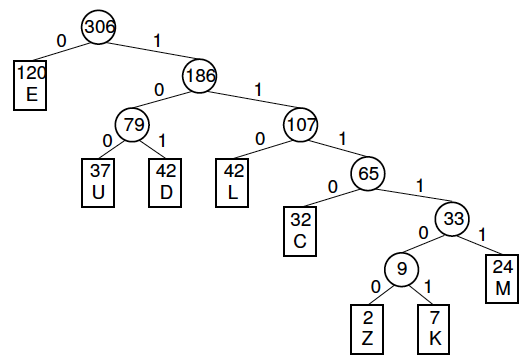
\includegraphics[width=10cm]{huffman_tree}
\end{center}

Decoding the Huffman tree is very simple, traverse the tree node by node as each bit is read from the input stream (reaching a leaf node necessarily terminates the search for that particular byte value). 

For example, decoding an encoded string can be done by looking at the bits in the coded string from left to right until a letter decoded.
10100101 $\Rightarrow$ DEED

\section{Lempel-Ziv(lz) Compression Methods}
Also known as the LZ family,it initially consisted of LZ-77 and LZ-78 which was published by Abraham Lempel and Jacob Ziv in 1977\cite{ziv1977universal} and 1978\cite{ziv1978compression}.Also known as LZ-1 and LZ-2 respectively,both are theoretically dictionary coders.These algorithms formed the basis for a lot of variations like LZW,LZSS,LZMA and also for a lot compression schemes like DEFLATE which has been discussed later in this article.
\subsection{LZ-77 Algorithm}
LZ77 algorithms achieve compression by replacing repeated occurrences of data with references to a copy of that data existing earlier within the uncompressed data stream. A match is encoded by a pair of numbers called a length-distance pair, which is like the statement "each of the next length characters is equal to the characters exactly distance characters behind it in the uncompressed stream".

To spot matches, the encoder must keep track of some amount of the recent data, like the last 2 kB, 4 kB, or 32 kB. The structure during which this data is held is named a sliding window , which is why LZ77 is usually called sliding-window compression. The encoder must keep this data to find matches, and therefore the decoder must keep this data to interpret the matches the encoder refers to. The larger the sliding window is, the longer back the encoder may look for creating references.

While encoding, for the search pointer to continue finding matched pairs after the end of the search window, all characters from the primary match at offset D and forward to the end of the search window must have matched input, and these are the (previously seen) characters that comprise one run unit of length LR, which must equal D. When search pointer proceeds past the search window and forward, as long as the run pattern repeats within the input, the search and input pointers are going to be in sync and match characters until the run pattern is interrupted. Then L characters had been matched in total, L > D, and therefore the code is [D, L, c].

Upon decoding [D, L, c], again, D = LR. When the primary LR characters are read to the output, this corresponds to one run unit appended to the output buffer. At this moment , the read pointer might be thought of as only needing to return int(L/LR) + (1 if L mod LR != 0) times to the beginning of that single buffered run unit, read LR characters (or maybe fewer on the last return), and repeat until all of the L characters are read. But mirroring the encoding process, since the pattern is repetitive, the read pointer need only trail in sync with the write pointer by a fixed distance which is equal to the run length LR until L characters are copied to output in total.

\textbf{Pseudocode}

\textbf{while} input not empty \textbf{do}

prefix : longest prefix of input that begins in window

\textbf{if} prefix exists \textbf{then}

j : distance to start of prefix

k : length of prefix

a : char following prefix in input

\textbf{else
}
j := 0

k := 0

a := first char of input

\textbf{end if}

\textbf{output} (j,k,a)

s := pop k + 1 chars from front of input

discard k + 1 chars from front of window

append s to back of window

\textbf{repeat}
\subsection{LZ-78 Algorithm}
The LZ78 is also a dictionary-based compression algorithm that maintains a dictionary. The encoded output
consists of two elements: an index pertaining to the longest matching lexical entry and therefore the first non-matching
symbol. The algorithm also adds the index and symbol pair to the dictionary. When the symbol is not yet found in
the dictionary, the codeword has the index value 0 and it's added to the dictionary as well . With this method, the
algorithm constructs the dictionary.
LZ78 algorithm has the power to capture patterns and hold them indefinitely but it also features a serious drawback.
The dictionary keeps growing forever without bound. There are a lot of methods to limit dictionary size. the
easiest one is to stop adding entries and continue like a static dictionary coder or to throw the dictionary away and
start from scratch after a certain number of entries has been reached\cite{zeeh2003lempel}

\textbf{Pseudocode}

q : NIL;

\textbf{While} (there is input) \textbf{do}{
	
	
	J : next symbol from input;
	
	\textbf{If} (qJ exists in the dictionary) \textbf{then} {
		
		q : qJ;
		
	}
	
	\textbf{Else} {
		
		\textbf{Output} (index(q), J);
		
		Add qJ to the dictionary;
		
		q : NIL;
		
	}\textbf{end if}
	
}\textbf{repeat}



\section{Arithmetic Coding}

Arithmetic coding is a data compression technique that encodes data (the data string) by creating a code string which represents a fractional value on the number line between 0 and 1. The coding algorithm is symbolwise recursive; i.e., it operates upon and encodes (decodes) one data symbol per iteration or recursion. On each recursion, the algorithm successively partitions an interval of the number line between 0 and 1, and retains one of the partitions as the new interval. Thus, the algorithm successively deals with smaller intervals, and the code string, viewed as a magnitude, lies in each of the nested intervals. The data string is recovered by using magnitude comparisons on the code string to recreate how the encoder must have successively partitioned and retained each nested subinterval. Arithmetic coding differs considerably from the more familiar compression coding techniques, such as prefix (Huffman) codes. Also, it should not be confused with error control coding, whose object is to detect and correct errors in computer operations.

\section{DEFLATE}

DEFLATE is a lossless data compression file format that uses a combination of LZSS and Huffman coding. It was designed by Phil Katz, for version 2 of his PKZIP archiving tool. Deflate was later specified in RFC 1951 (1996). Katz also designed the original algorithm used to construct Deflate streams. This algorithm was patented as U.S. Patent 5,051,745, and assigned to PKWARE, Inc.[2][3] As stated in the RFC document, an algorithm producing Deflate files was widely thought to be implementable in a manner not covered by patents.[1] This led to its widespread use, for example in gzip compressed files and PNG image files, in addition to the ZIP file format for which Katz originally designed it.

\vspace{0.3in}

\textbf{\Large{Current Research Work}}

The current research work in Data Compression has shifted more towards the application part, where data compression is being applied in all sorts of fields like Deep Learning, Networking, Image Compression, Video and Audio Compression etc. We have discussed few papers which represent the research done in various domains to get the most out of data compression and make computing systems more efficient.

\section{Tweet Classification By Data Compression \cite{10.1145/2064448.2064473}}

The above mentioned paper proposes a compression based method for classification of tweets. They used the DEFLATE algorithm to compress the tweet and then evaluate and classify the given tweet according to its compressibility. The proposed method achieved higher accuracy when compared to the state of the art learning methods. 

\subsection{Proposed Method}

The main problem was to classify the tweet according to the sentiment of the tweet, i.e classifying them into "positive" and "negative" classes. The algorithm was fed query strings and then slow it learns the difference by creating two tweet models $M_n$ and $M_p$. Finally the algorithm calculates a classification score $f(x)$ which is then used to finally classify using a fixed threshold value.

\subsection{Classification}

There are 2 steps involved in the classification procedure. The first step calculated the compressibility of the tweet and the second step calculates the classification score. \\ 

The Compressibility scores are calculated as follows  \cite{10.1145/2064448.2064473}

$$C_p = Z(M_p . x) - Z(M_p)$$
$$C_n = Z(M_n . x) - Z(M_n)$$

Where $C_p$ and $C_n$ are the compressibility scores. $M_p . x$ implies that $x$ is appended to $M_p$ and $Z(k)$ is the compressed size of the input $k$ 

And finally the classification score is calculated as follows

$$
f(x) = \frac{C_p(x) + \gamma}{C_n(x) + \gamma}
$$

where $\gamma$ is a smoothing parameter. Also known as Laplace Smoothing. 

\subsection{Results}

According to the results mentioned in the article, CTC performed statistically better than the state of the art methods. This method also applies to multi lingual tweets which gives it an edge over some of the other machine learning approaches.

This paper was an interesting application of the DEFLATE algorithm to classify tweets.


\section{Energy Aware Lossless Data Compression \cite{10.1145/1151690.1151692}}

This paper reports a rather different viewpoint on the whole compression domain. The energy required to send a bit via wireless transmission is close to 1000 times higher than the energy required for a regular 32 bit operation on a computer. The article reports the fact that compressing and decompressing information before and after transmission is more energy expensive compared to the case without any compression. The paper suggests solutions to this problem and they are able to achive an energy reduction of close to 51\%.

\subsection{Methodologies and Summary}
The tests were done on a Compaq Personal Server codenamed "Skiff". 

The energy required for compression and decompression are almost directly proportional to time required for executing. The energy required is observed to be more for aggressively compressed data due to the large number of memory references. Even though the energy requirement is proportional to the execution time, using the fastest algorithm for compression and decompression doesn't reduce the energy footprint. They were able to conclude the fact that reducing energy is not as simple as picking the fastest compression algorithm.

The energy requirements of the CPU and Network change drastically. They are extremely difficult to predict over a period of time. Thus software developers have to be aware of their hardware constraints and optimize accordingly to reduce energy footprint. 

\section{Lossless Compression of Already Compressed Textures \cite{strom2011lossless}}

The following cited paper investigates and proposes a lossless compression algorithm for rendering textures in graphics

Compressing textures allow the computer to render more textures due to smaller memory consumption, as the memory access. Compared to image compression methods like JPEG however, textures codecs are typically much less efficient, which is a problem when downloading the texture over a network or reading it from disk. Therefore, in this paper we investigate lossless compression of already compressed textures. By predicting compression parameters in the image domain instead of in the parameter domain, a more efficient representation is obtained compared to using general compression such as ZIP or LZMA.

\section{Texture compression using low-frequency signal modulation \cite{10.5555/844174.844187}}

A new lossy texture compression technique is presented in this paper that is suited to implementation on low-cost, low-bandwidth devices as well as more powerful rendering systems. It uses a representation that is based on the blending of two (or more) 'low frequency' signals using a high frequency but low precision modulation signal. Continuity of the low frequency signals helps to avoid block artifacts. Decompression costs are kept low through use of fixed-rate encoding and by eliminating indirect data access.

Some of the other interesting papers we found are cited below.

\textbf{Towards Analysis-friendly Face Representation with Scalable Feature and Texture Compression \cite{wang2020towards}}

\textbf{On the Compressive Power of Boolean Threshold Autoencoders \cite{melkman2020compressive}}

\section{Conclusion and Future Prospects}

In the presented review article we had an overview and simple examples of some of the most established methods in the domain of Lossless Data Compression. We also had a look at some of the modern research going on in the field. Almost every software system in function today has a component of compression and decompression to reduce the load and improve efficiency. 

As we are moving towards a more data driven age, the amount of which users are creating data is exploding. In such scenarios, data compression stands at a very crucial juncture. Active research in this field will yield astonishing speed improvements in the current computing landscape.

\clearpage

\bibliographystyle{unsrt}
\bibliography{main}


\textbf{Review References}

\begin{enumerate}
	\setcounter{enumi}{17}
	
	\item D. Benedetto, E. Caglioti, and V. Loreto. Language
	trees and zipping. Physical Review Letters, 88(4), 28
	Jan. 2002.
	
	\item A. Bratko, G. V. Cormack, B. Filipi˘c, T. R. Lynam,
	and B. Zupan. Spam filtering using statistical data
	compression models. Journal of Machine Learning
	Research, 7:2673–2698, 2006.
	
	\item M. Burrows and D. J. Wheeler. A block-sorting
	lossless data compression algorithm. Technical Report
	SRC-RR-124, Digiral Systems Research Center, 1994.
	
	\item R. Cilibrasi and P. Vit´anyi. Clustering by
	compression. IEEE Transactions on Information
	Theory, 51(4):1523–1545, 2005.
	
	\item J. G. Cleary and I. H. Witten. Data compression using
	adaptive coding and partial string matching. IEEE
	Transactions on Communications,
	COM-32(4):396–402, 1984.
	
	\item G. Cormack and R. N. S. Horspool. Data compression
	using dynamic markov modelling. The Computer
	Journal, 30(6):541–550, 1987.
	
	\item K. Crammer, O. Dekel, J. Keshet, S. Shalev-Shwartz,
	and Y. Singer. Online passive-agressive algorithm.
	Journal of Machine Learning Research, 7:551–585,
	2006.

	\item M. Dredze, K. Crammer, and F. Pereira.
	Confidence-weighted linear classification. In
	Proceedings of 25th International Conference on
	Machine Learning, pages 264–271, 2008.

	\item D. Irani, S. Webb, C. Pu, and K. Li. Study of
	trend-stuffing on twitter through text classification. In
	Proceedings of 7th Annual Collaboration, Electronic
	messaging, Anti-Abuse and Spam Conference, 2010.

	\item H. Kwak, C. Lee, H. Park, and S. Moon. What is
	twitter, a social network or a news media? In
	Proceedings of 19th International Conference on
	World Wide Web, pages 591–600, 2010.

	\item M. Li, X. Chen, X. Li, B. Ma, and P. M. B. Vit´anyi.
	The similarity metric. IEEE Transactions on
	Information Theory, 50(12):3250–3264, 2004.

	\item M. Li and P. Vit´anyi. An Introduction to Kolmogorov
	Complexity and Its Applications. Springer, 2nd
	edition, 1997.

	\item Y. Marton, N. Wu, and L. Hellerstein. On
	compression-based text classification. In Proceedings of
	the 27th European Conference on Information
	Retrieval, pages 300–314, 2005.
	
	\item T. Sakaki, M. Okazaki, and Y. Matsuo. Earthquake
	shakes twitter users: Real-time event detection by
	social sensors. In Proceedings of 19th International
	Conference on World Wide Web, pages 851–860, 2010.
	
	\item B. Sriram, D. Fuhry, and M. Demirbas. Short text
	classification in twitter to improve information
	filtering. In Proceedings of 33rd International ACM
	SIGIR Conference on Research and Development in
	Information Retrieval, pages 841–842, 2010.
	
	\item I. H. Witten, A. Moffat, and T. C. Bell. Managing
	Gigabytes: compressing and indexing documents and
	images. Morgan Kaufmann, 2nd edition, 1999.

	\item J. Ziv and A. Lempel. A universal algorithm for
	sequential data compression. IEEE Transactions on
	Information Theory, IT-23(3):337–343, 1977.
	
	\item Advanced RISC Machines Ltd (ARM). Writing Efficient
	C for ARM, Jan. 1998. Application Note 34.
	
	\item T. M. Austin and D. C. Burger. SimpleScalar version 4.0
	release. Tutorial in conjunction with 34th Annual International Symposium on Microarchitecture, Dec. 2001.
	
	\item T. Bell and D. Kulp. Longest match string searching for
	Ziv-Lempel compression. Technical Report 06/89, Department of Computer Science, University of Canterbury,
	New Zealand, 1989.
	
	\item T. Bell, M. Powell, J. Horlor, and R. Arnold. The Canterbury Corpus. http://www.corpus.canterbury.ac.nz/.

	\item T. Bell, I. H. Witten, and J. G. Cleary. Modeling for text
	compression. ACM Computing Surveys, 21(4):557–591,
	1989.

	\item J. Bilmes, K. Asanovic, C.-W. Chin, and J. Demmel. Op- ´
	timizing matrix multiply using PHiPAC: a portable, highperformance, ANSI C coding methodology. In 11th ACM
	International Conference on Supercomputing, July 1997.
	
	\item D. C. Burger and T. M. Austin. The SimpleScalar tool
	set, version 2.0. Technical Report CS-TR-97-1342, University of Wisconsin, Madison, June 1997.
	
	\item M. Burrows and D. J. Wheeler. A block-sorting lossless
	data compression algorithm. Technical Report 124, Digital Systems Research Center, May 1994.
	
	\item J. Gailly and M. Adler. zlib. http://www.gzip.org/zlib.
	
	\item J. Gailly, Maintainer. comp.compression Internet
	newsgroup: Frequently Asked Questions, Sept. 1999.

	\item J. Gilchrist. Archive comparison test.
	http://compression.ca.
	
	\item P. J. Havinga. Energy efficiency of error correction on
	wireless systems. In IEEE Wireless Communications and
	Networking Conference, Sept. 1999.
	
	\item J. Hicks et al. Compaq personal server
	project, 1999. http://crl.research.compaq.com
	/projects/personalserver/default.htm.

	\item B. C. Housel and D. B. Lindquist. Webexpress: a system
	for optimizing web browsing in a wireless environment.
	In Proceedings of the Second Annual International Conference on Mobile Computing and Networking, 1996.

	\item J. J. Hunt, K.-P. Vo, and W. F. Tichy. An empirical study
	of delta algorithms. In Software configuration management: ICSE 96 SCM-6 Workshop. Springer, 1996.

	\item Hyperspace Communications, Inc.
	Mod gzip. http://www.ehyperspace.com /htmlonly/products/mod gzip.html.

	\item Intel Corporation. SA-110 Microprocessor Technical Reference Manual, December 2000.


	\item Intel Corporation. Intel StrongARM SA-1110 Microprocessor Developer’s Manual, October 2001.

	\item V. Jacobson. RFC 1144: Compressing TCP/IP headers
	for low-speed serial links, Feb. 1990.

	\item K. Jamieson. Implementation of a power-saving protocol for ad hoc wireless networks. Master’s thesis, Massachusetts Institute of Technology, Feb. 2002.

	\item P. Jannesen et. al. (n)compress. available, among other
	places, in Redhat 7.2 distribution of Linux.

	\item K. Koskelin, K. Barr, and K. Asanovic. Eprof: An en- ´
	ergy profiler for the iPaq. In 2nd Annual Student Oxygen
	Workshop. MIT Project Oxygen, 2002.

	\item R. Krashinsky. Efficient web browsing for mobile clients
	using HTTP compression. Technical Report MIT-LCSTR-882, MIT Lab for Computer Science, Jan. 2003.

	\item J. Lilley, J. Yang, H. Balakrishnan, and S. Seshan. A unified header compression framework for low-bandwidth
	links. In 6th ACM MOBICOM, Aug. 2000.

	\item Lycos. Lycos 50, Sept. 2002. Top 50 searches on Lycos
	for the week ending September 21, 2002.

	\item A. Miyoshi, C. Lefurgy, E. V. Hensbergen, R. Rajamony,
	and R. Rajkumar. Critical power slope: Understanding
	the runtime effects of frequency scaling. In International
	Conference on Supercomputing, June 2002.

	\item J. C. Mogul. Trace-based analysis of duplicate suppression in HTTP. Technical Report 99.2, Compaq Computer
	Corporation, Nov. 1999.

	\item J. C. Mogul, F. Douglis, A. Feldmann, and B. Krishnamurthy. Potential benefits of delta encoding and data
	compression for HTTP. Technical Report 97/4a, Compaq Computer Corporation, Dec. 1997.

	\item J. Montanaro et al. A 160-mhz, 32-b, 0.5-w CMOS RISC
	microprocessor. IEEE Journal of Solid-State Circuits,
	31(11), Nov. 1996.

	\item N. Motgi and A. Mukherjee. Network conscious text
	compression systems (NCTCSys). In Proceedings of
	International Conference on Information and Theory:
	Coding and Computing, 2001.

	\item A. Muthitacharoen, B. Chen, and D. Mazi`eres. A lowbandwidth network file system. In Proceedings of the
	18th ACM Symposium on Operating Systems Principles (SOSP ’01), pages 174–187, Chateau Lake Louise,
	Banff, Canada, October 2001.

	\item Nielsen NetRatings Audience Measurement Service. Top
	25 U.S Properties; Week of Sept 15th., Sept. 2002.
	
	\item M. F. Oberhumer. LZO.
	http://www.oberhumer.com/opensource/lzo/.

	\item A. Peymandoust, T. Simuni ˘ c, and G. D. Micheli. Low ´
	power embedded software optimization using symbolic
	algebra. In Design, Automation and Test in Europe, 2002.

	\item J. Santos and D. Wetherall. Increasing effective link
	bandwidth by suppressing replicated data. In USENIX
	Annual Technical Conference, June 1998.

	\item K. Sayood. Introduction to data compression. Morgan
	Kaufman Publishers, second edition, 2002.

	\item J. Seward. bzip2. http://www.spec.org
	/osg/cpu2000/CINT2000/256.bzip2/docs/256.bzip2.html.

	\item J. Seward. e2comp bzip2 library.
	http://cvs.bofh.asn.au/e2compr/index.html.

	\item A. Shacham, B. Monsour, R. Pereira, and M. Thomas.
	RFC 3173: IP payload compression protocol, Sept. 2001.

	\item D. Shkarin. PPMd.
	ftp://ftp.elf.stuba.sk/pub/pc/pack/ppmdi1.rar.

	\item A. Sinha, A. Wang, and A. Chandrakasan. Algorithmic
	transforms for efficient energy scalable computation. In
	IEEE International Symposium on Low Power Electronics and Design, August 2000.

	\item Standard Performance Evaluation Corporation.
	CPU2000, 2000.

	\item C. N. Taylor and S. Dey. Adaptive image compression
	for wireless multimedia communication. In IEEE International Conference on Communication, June 2001.

	\item A. Tridgell. Efficient Algorithms for Sorting and Synchronization. PhD thesis, Australian National University,
	Apr. 2000.

	\item T. Simuni ˘ c, L. Benini, and G. D. Micheli. Energy- ´
	efficient design of battery-powered embedded systems.
	In IEEE International Symposium on Low Power Electronics and Design, 1999.

	\item T. Simuni ˘ c, L. Benini, G. D. Micheli, and M. Hans. ´
	Source code optimization and profiling of energy consumption in embedded systems. In International Symposium on System Synthesis, 2000.

	\item M. A. Viredaz and D. A. Wallach. Power evaluation of
	Itsy version 2.4. Technical Report TN-59, Compaq Computer Corporation, February 2001.

	\item H. Yang, G. R. Gao, A. Marquez, G. Cai, and Z. Hu.
	Power and energy impact of loop transformations. In
	Workshop on Compilers and Operating Systems for
	Low Power 2001, Parallel Architecture and Compilation
	Techniques, Sept. 2001.
	
	\item BEERS, A., AGRAWALA, M., AND CHADDA, N. 1996. Rendering
	from Compressed Textures. In Proceedings of ACM SIGGRAPH
	96, 373–378.

	\item BPTC, 2010. ARB texture compression bptc. Available online:
	www.opengl.org/registry/specs/ARB/texture compression bptc.txt.

	\item CAMPBELL, G., DEFANTI, T. A., FREDERIKSEN, J., JOYCE,
	S. A., LESKE, L. A., LINDBERG, J. A., AND SANDIN, D. J.
	1986. Two Bit/Pixel Full Color Encoding. In Computer Graphics (Proceedings of ACM SIGGRAPH 86), 215–223.
	
	\item DELP, E. J., AND MITCHELL, O. R. 1979. Image Compression
	using Block Truncation Coding. IEEE Transactions on Communications 2, 9, 1335–1342.

	\item FENNEY, S. 2003. Texture Compression using Low-Frequency
	Signal Modulation. In Graphics Hardware, ACM Press, 84–91.
	INADA, T., AND MCCOOL, M. 2006. Compressed Lossless Texture Representation and Caching. In Graphics Hardware, 111–	120.

	\item IOURCHA, K., NAYAK, K., AND HONG, Z., 1999. System and
	Method for Fixed-Rate Block-Based Image Compression with
	Inferred Pixel Values. US Patent 5,956,431.	
	
	\item JPEG, 2000. JPEG 2—ISO/IEC 15444-1:2005. Available online:http://www.jpeg.org/jpeg2000/.
	
	\item KNITTEL, G., SCHILLING, A. G., KUGLER, A., AND STRASSER, W. 1996. Hardware for Superior Texture Performance. Computers and Graphics, 20, 4, 475–481.
	
	\item MICROSOFT, 2006. HD Photo. Available online:
	http:/www.microsoft.com/windows/windowsmedia/forpros/
	wmphoto/default.aspx.

	\item OWENS, J. D. 2005. Streaming Architectures and Technology
	Trends. In GPU Gems 2. Addison-Wesley, 457–470.

	\item RASMUSSON, J., STROM¨ , J., WENNERSTEN, P., DOGGETT,
	M., AND AKENINE-MOLLER ¨ , T. 2010. Texture Compression of Light Maps using Smooth Profile Functions. In HighPerformance Graphics, 143–152.

	\item STROM¨ , J., AND AKENINE-MOLLER ¨ , T. 2005. iPACKMAN:
	High-Quality, Low-Complexity Texture Compression for Mobile Phones. In Graphics Hardware, 63–70.
	\item STROM¨ , J., AND PETTERSSON, M. 2007. ETC2: Texture Compression using Invalid Combinations. In Graphics Hardware,
	49–54.
	
	\item SUEHRING ¨ , K. 2009. JM Software H.264/AVC.
	http://iphome.hhi.de/suehring/tml/.
	TORBORG, J., AND KAJIYA, J. 1996. Talisman: Commodity Realtime 3D Graphics for the PC. In Proceedings of SIGGRAPH,
	353–364.
	
	\item VAN WAVEREN, J., 2006. Real-Time Texture Streaming and
	Decompression. Id Software Technical Report, available at
	http://software.intel.com/file/17248/.
	\item WEINBERGER, M., SEROUSSI, G., AND SAPIRO, G. 1996.
	LOCO-I: A Low Complexity, Context-Based, Lossless Image
	Compression Algorithm. In Proc. IEEE Data Compression Conference, Snowbird, Utah, March-April 1996.
	
	\item WHEELER, F., 1996. Adaptive Arithmetic Coding Source Code.
	available at http://www.cipr.rpi.edu/ wheeler/ac/.
	
	\item WITTEN, I. H., NEAL, R. M., AND CLEARY, J. G. 1987. Arithmetic Coding for Data Compression. Communications of the	ACM 30, 6.
	
	\item Edwin Catmull. “Computer Display of Curved Surfaces”, Proc. IEEE Conf. Computer Graphics, Pattern Recognition, and Data Structures May 1975, 11–17.

	\item Andrew C. Beers, Maneesh Agrawala, and Navin
	Chadda. “Rendering from Compressed Textures”,
	Computer Graphics, Proc. SIGGRAPH 7(3),
	Aug.1996, 373–378

	\item James Kajiya, Ivan Sutherland, and Edward Cheadle.
	“A Random-Access Video Frame Buffer”, Proc. IEEE
	Computer Graphics, Pattern Recognition, and Data
	Structures May 1975, 1–6.

	\item Paul Heckbert. “Color Image Quantisation for Frame
	Buffer Display”, Computer Graphics 16(3), July 1982,
	297–307.
	
	\item Xiaolin Wu. “Color Quantization by Dynamic Programming and Principal Analysis”, ACM Transactions
	on Graphics 11(4), Oct. 1992, 348–372.
	
	\item Lance Williams. “Pyramidal Parametrics”, Computer
	Graphics 7(3), July 1983, 1–11.
	
	\item E. Delp and O. Mitchell. “Image Compression Using
	Block Truncation Coding”, IEEE Trans. on Communications. Vol.COM-2 (9), Sept. 1979, 1335–1342.

	\item Graham Campbell et al. “Two bit/pixel full color encoding”, Computer Graphics 20(4), August 1986, 215–
	223.

	\item G. Knittel, A. Schilling, A. Kugler, and W. Strasser.
	“Hardware for Superior Texture Performance”, Proceedings of the 10th Eurographics Workshop on Graphics Hardware 1995, 33–39.

	\item Konstantine Iourcha, Krishna Nayak, and Zhou Hong.
	“System and Method for Fixed-Rate Block-Based Image Compression with Inferred Pixel Values”, US
	Patent 5,956,431.

	\item L. Levkovich-Maslyuk, P. G. Kalyuzhny, and A.
	Zhirkov. “Texture Compression with Adaptive Block
	Partitions”, ACM Multimedia 2000 Nov. 2000.

	\item A.V. Pereberin. “Hierarchical Approach for Texture Compression”, Proceedings of GraphiCon ‘99
	1999,195–199.
	
	\item Denis Ivanov and Yevgeniy Kuzmin. “Color Distribution - A New Approach to Texture Compression”, Computer Graphics Forum 19(3), August 2000, 283–289.
	
	\item Eric Stollnitz, Tony DeRose, and David Salesin.
	“Wavelets for Computer Graphics. Theory and Applications”, ISBN 1-55860-375-1
	\item Wim Sweldens and Peter Shroeder. “Building your own
	Wavelets at Home”, Journal Technical Report 1995:5,	Industrial Mathematics Initiative, Department of Mathematics, University of South Carolina

	\item Press, Teukolsky, Vettering, and Flannery. “Numerical
	Recipes in C”, ISBN 0-521-43108-5
	
	\item http://sqez.home.att.net/thumbs/Thumbnails.html
	
	\item G. K. Wallace, “The JPEG still picture compression standard,” IEEE
	Transactions on Consumer Electronics, vol. 38, no. 1, pp. xviii–xxxiv,
	1992.
	
	\item M. Rabbani, “JPEG2000: Image compression fundamentals, standards
	and practice,” Journal of Electronic Imaging, vol. 11, no. 2, p. 286,
	2002.
	
	\item T. Wiegand, G. J. Sullivan, G. Bjontegaard, and A. Luthra, “Overview of
	the H. 264/AVC video coding standard,” IEEE Transactions on Circuits
	and Systems for Video Technology, vol. 13, no. 7, pp. 560–576, 2003.
	
	\item G. J. Sullivan, J.-R. Ohm, W.-J. Han, and T. Wiegand, “Overview of the
	high efficiency video coding (HEVC) standard,” IEEE Transactions on
	Circuits and Systems for Video Technology, vol. 22, no. 12, pp. 1649–
	1668, 2012.
	
	\item A. Mohan, K. Gauen, Y.-H. Lu, W. W. Li, and X. Chen, “Internet
	of video things in 2030: A world with many cameras,” in IEEE
	International Symposium on Circuits and Systems. IEEE, 2017, pp.
	1–4.
	
	\item L.-Y. Duan, V. Chandrasekhar, J. Chen, J. Lin, Z. Wang, T. Huang,
	B. Girod, and W. Gao, “Overview of the MPEG-CDVS standard,” IEEE
	Transactions on Image Processing, vol. 25, no. 1, pp. 179–194, 2015.
	
	\item L.-Y. Duan, Y. Lou, Y. Bai, T. Huang, W. Gao, V. Chandrasekhar, J. Lin,
	S. Wang, and A. C. Kot, “Compact descriptors for video analysis: The
	emerging MPEG standard,” IEEE MultiMedia, vol. 26, no. 2, pp. 44–54,
	2018.
	
	\item L.-Y. Duan, J. Liu, W. Yang, T. Huang, and W. Gao, “Video coding
	for machines: A paradigm of collaborative compression and intelligent
	analytics,” arXiv preprint arXiv:2001.03569, 2020.	

	\item Y. Li, C. Jia, S. Wang, X. Zhang, S. Wang, S. Ma, and W. Gao, “Joint
	rate-distortion optimization for simultaneous texture and deep feature
	compression of facial images,” in 2018 IEEE Fourth International
	Conference on Multimedia Big Data. IEEE, 2018, pp. 1–5.

	\item S. Wang, S. Wang, X. Zhang, S. Wang, S. Ma, and W. Gao, “Scalable
	facial image compression with deep feature reconstruction,” in 2019
	IEEE International Conference on Image Processing. IEEE, 2019, pp.
	2691–2695.

	\item I. Recommendation, “Generic coding of moving pictures and associated
	audio information: Video,” 1995.

	\item J. Pfaff, B. Stallenberger, M. Schafer, P. Merkle, P. Helle, T. Hinz,
	H. Schwarz, D. Marpe, and T. Wiegand, “CE3: Affine linear weighted
	intra prediction (CE3–4.1 CE3–4.2),” in document JVET-N0217, in Proc.
	of 14th JVET meeting, 2019.

	\item J. An, Y. Chen, K. Zhang, H. Huang, Y. Huang, and S. Lei, “Block
	partitioning structure for next generation video coding,” MPEG doc.
	m37524 and ITU-T SG16 Doc. COM16–C966, 2015.

	\item M. Wang, J. Li, L. Zhang, K. Zhang, H. Liu, S. Wang, S. Kwong,
	and S. Ma, “Extended coding unit partitioning for future video coding,”
	IEEE Transactions on Image Processing, 2019.

	\item S. Lin, H. Chen, H. Zhang, S. Maxim, H. Yang, and J. Zhou, “Affine
	transform prediction for next generation video coding,” MPEG doc.
	m37525 and ITU-T SG16 Doc. COM16–C1016, 2015.

	\item X. Chen, J. An, and J. Zheng, “EE3: Decoder-side motion vector refinement based on bilateral template matching,” in Joint Video Exploration
	Team of ITU-T SG16 WP3 and ISO/IEC JTC1/SC29/WG11, JVETE0052, 5th Meeting, 2017.

	\item X. Zhao, J. Chen, and M. Karczewicz, “Mode-dependent non-separable
	secondary transform,” ITU-T SG16/Q6 Doc. COM16–C1044, 2015.

	\item B. Li, H. Li, L. Li, and J. Zhang, “Lambda domain rate control algorithm for
	high efficiency video coding,” IEEE Transactions on Image Processing,
	vol. 23, no. 9, pp. 3841–3854, 2014.

	\item J. Chao, R. Huitl, E. Steinbach, and D. Schroeder, “A novel rate control
	framework for SIFT/SURF feature preservation in H. 264/AVC video
	compression,” IEEE Transactions on Circuits and Systems for Video
	Technology, vol. 25, no. 6, pp. 958–972, 2014.

	\item T. Huang, “Surveillance video: The biggest big data,” Computing Now,
	vol. 7, no. 2, pp. 82–91, 2014.

	\item M. Paul, W. Lin, C.-T. Lau, and B.-S. Lee, “Explore and model better
	i-frames for video coding,” IEEE Transactions on Circuits and Systems
	for Video Technology, vol. 21, no. 9, pp. 1242–1254, 2011.

	\item X. Zhang, T. Huang, Y. Tian, and W. Gao, “Background-modeling-based
	adaptive prediction for surveillance video coding,” IEEE Transactions
	on Image Processing, vol. 23, no. 2, pp. 769–784, 2013.

	\item F. Chen, H. Li, L. Li, D. Liu, and F. Wu, “Block-composed background
	reference for high efficiency video coding,” IEEE Transactions on
	Circuits and Systems for Video Technology, vol. 27, no. 12, pp. 2639–
	2651, 2016.

	\item H. Yue, X. Sun, J. Yang, and F. Wu, “Cloud-based image coding for mobile devicestoward thousands to one compression,” IEEE Transactions
	on Multimedia, vol. 15, no. 4, pp. 845–857, 2013.

	\item Z. Shi, X. Sun, and F. Wu, “Photo album compression for cloud storage
	using local features,” IEEE Journal on Emerging and Selected Topics
	in Circuits and Systems, vol. 4, no. 1, pp. 17–28, 2014.
	
	\item L. Zhao, Z. He, W. Cao, and D. Zhao, “Real-time moving object segmentation and classification from hevc compressed surveillance video,” IEEE
	Transactions on Circuits and Systems for Video Technology, vol. 28,
	no. 6, pp. 1346–1357, 2016.

	\item D. Edmundson and G. Schaefer, “An overview and evaluation of JPEG
	compressed domain retrieval techniques,” in Proceedings ELMAR-2012.
	IEEE, 2012, pp. 75–78.

	\item G. Toderici, S. M. O’Malley, S. J. Hwang, D. Vincent, D. Minnen,
	S. Baluja, M. Covell, and R. Sukthankar, “Variable rate image compression with recurrent neural networks,” ICLR, 2016.

	\item J. Balle, V. Laparra, and E. Simoncelli, “End-to-end optimized image ´
	compression,” in International Conference on Learning Representations,
	2017.

	\item J. Balle, D. Minnen, S. Singh, S. J. Hwang, and N. Johnston, “Variational ´image compression with a scale hyperprior,” in International Conference
	on Learning Representations, 2018.

	\item G. Lu, W. Ouyang, D. Xu, X. Zhang, C. Cai, and Z. Gao, “DVC: An
	end-to-end deep video compression framework,” in Proceedings of the
	IEEE Conference on Computer Vision and Pattern Recognition, 2019,
	pp. 11 006–11 015.

	\item A. Redondi, L. Baroffio, M. Cesana, and M. Tagliasacchi, “Compressthen-analyze vs. analyze-then-compress: Two paradigms for image analysis in visual sensor networks,” in IEEE International Workshop on
	Multimedia Signal Processing. IEEE, 2013, pp. 278–282.

	\item W. Liu, J. Wang, R. Ji, Y.-G. Jiang, and S.-F. Chang, “Supervised
	hashing with kernels,” in 2012 IEEE Conference on Computer Vision
	and Pattern Recognition. IEEE, 2012, pp. 2074–2081.

	\item V. Chandrasekhar, G. Takacs, D. Chen, S. S. Tsai, J. Singh, and
	B. Girod, “Transform coding of image feature descriptors,” in Visual
	Communications and Image Processing 2009, vol. 7257. International
	Society for Optics and Photonics, 2009, p. 725710.

	\item H. Jegou, M. Douze, and C. Schmid, “Product quantization for nearest
	neighbor search,” IEEE Transactions on Pattern Analysis and Machine
	Intelligence, vol. 33, no. 1, pp. 117–128, 2010.

	\item A. Krizhevsky, I. Sutskever, and G. E. Hinton, “Imagenet classification
	with deep convolutional neural networks,” in Advances in Neural Information Processing Systems, 2012, pp. 1097–1105.

	\item K. Simonyan and A. Zisserman, “Very deep convolutional networks for
	large-scale image recognition,” in International Conference on Learning
	Representations, 2015.

	\item F. Schroff, D. Kalenichenko, and J. Philbin, “Facenet: A unified embedding for face recognition and clustering,” in Proceedings of the IEEE
	Conference on Computer Vision and Pattern Recognition, 2015, pp. 815–
	823.

	\item L. Ding, Y. Tian, H. Fan, Y. Wang, and T. Huang, “Rate-performanceloss optimization for inter-frame deep feature coding from videos,” IEEE
	Transactions on Image Processing, vol. 26, no. 12, pp. 5743–5757, 2017.

	\item L. Ding, Y. Tian, H. Fan, C. Chen, and T. Huang, “Joint coding of local
	11
	and global deep features in videos for visual search,” IEEE Transactions
	on Image Processing, vol. 29, pp. 3734–3749, 2020.

	\item H. Zhu, M. Long, J. Wang, and Y. Cao, “Deep hashing network for
	efficient similarity retrieval,” in Thirtieth AAAI Conference on Artificial
	Intelligence, 2016.

	\item S. Wang, W. Yang, and S. Wang, “End-to-end facial deep learning
	feature compression with teacher-student enhancement,” arXiv preprint
	arXiv:2002.03627, 2020.

	\item Z. Chen, K. Fan, S. Wang, L. Duan, W. Lin, and A. C. Kot, “Toward
	intelligent sensing: Intermediate deep feature compression,” IEEE Transactions on Image Processing, vol. 29, pp. 2230–2243, 2020.

	\item Y. Hu, S. Yang, W. Yang, L.-Y. Duan, and J. Liu, “Towards coding for
	human and machine vision: A scalable image coding approach,” arXiv
	preprint arXiv:2001.02915, 2020.

	\item S. Xia, K. Liang, W. Yang, L.-Y. Duan, and J. Liu, “An emerging coding
	paradigm VCM: A scalable coding approach beyond feature and signal,”
	arXiv preprint arXiv:2001.03004, 2020.

	\item Y. Lou, L. Duan, S. Wang, Z. Chen, and W. Gao, “Front-end smart visual
	sensing and back-end intelligent analysis: A unified infrastructure for
	economizing the visual system of city brain,” IEEE Journal on Selected
	Areas in Communications, vol. PP, no. 99, pp. 1–1, 2019.

	\item L. Duan, Y. Lou, S. Wang, W. Gao, and Y. Rui, “AI-oriented largescale video management for smart city: Technologies, Standards, and
	Beyond,” IEEE MultiMedia, vol. 26, no. 2, pp. 8–20, April 2019.

	\item G. Wen, Y. Tian, T. Huang, S. Ma, and X. Zhang, “The IEEE 1857
	standard: Empowering smart video surveillance systems,” Intelligent
	Systems IEEE, vol. 29, no. 5, pp. 30–39, 2014.

	\item Y. Lou, L. Duan, Y. Luo, Z. Chen, T. Liu, S. Wang, and W. Gao,
	“Towards efficient front-end visual sensing for digital retina: A modelcentric paradigm,” IEEE Transactions on Multimedia, 2020.

	\item C. Szegedy, S. Ioffe, V. Vanhoucke, and A. A. Alemi, “Inception-v4,
	Inception-Resnet and the impact of residual connections on learning,”
	in Thirty-first AAAI conference on artificial intelligence, 2017.

	\item B. Gary, R. Manu, B. Tamara, and L. Erik, “Labeled faces in the wild: A
	database for studying face recognition in unconstrained environments,”
	University of Massachusetts, Amherst, Tech. Rep. 07-49, October 2007.

	\item Q. Cao, L. Shen, W. Xie, O. Parkhi, and A. Zisserman, “VGGFace2:
	A dataset for recognising faces across pose and age,” in International
	Conference on Automatic Face and Gesture Recognition, 2018.

	\item S. Ma, X. Zhang, C. Jia, Z. Zhao, S. Wang, and S. Wanga, “Image and
	video compression with neural networks: A review,” IEEE Transactions
	on Circuits and Systems for Video Technology, 2019.

	\item X. Glorot and Y. Bengio, “Understanding the difficulty of training
	deep feedforward neural networks,” in Proceedings of the Thirteenth
	International Conference on Artificial Intelligence and Statistics, 2010,
	pp. 249–256.

	\item D. Kingma and J. Ba, “Adam: A method for stochastic optimization,”
	arXiv preprint arXiv:1412.6980, 2014.

	\item K. Zhang, Z. Zhang, Z. Li, and Y. Qiao, “Joint face detection and
	alignment using multitask cascaded convolutional networks,” IEEE
	Signal Processing Letters, vol. 23, no. 10, pp. 1499–1503, 2016.

	\item H. Jgou, M. Douze, and C. Schmid, “Product quantization for nearest
	neighbor search,” IEEE Transactions on Pattern Analysis and Machine
	Intelligence, vol. 33, no. 1, pp. 117–128, Jan 2011.

	\item T. Ge, K. He, Q. Ke, and J. Sun, “Optimized product quantization,” IEEE
	Transactions on Pattern Analysis and Machine Intelligence, vol. 36,
	no. 4, pp. 744–755, April 2014.

	\item W. Liu, J. Wang, R. Ji, Y. Jiang, and S. Chang, “Supervised hashing
	with kernels,” in 2012 IEEE Conference on Computer Vision and Pattern
	Recognition, June 2012, pp. 2074–2081.
	
	\item D. H. Ackley, G. H. Hinton, and T. J. Sejnowski, “A learning algorithm for Boltzmann machines,” Cognitive Science, vol. 9, pp. 147–169, 1985.

	\item P. Baldi and K. Hornik, “Neural networks and principal component analysis: Learning from
	examples without local minima,” Neural Networks, vol. 2, pp. 53–38, 1989.

	\item G. E. Hinton and R. R. Salakhutdinov, “Reducing the dimensionality of data with neural
	networks,” Science, vol, 313, pp. 504–507, Jul. 2006.

	\item P. Baldi, “Autoencoders, unsupervised learning, and deep architectures,” JMLR: Workshop
	and Conference Proceedings, vol. 27, pp. 37–50, 2012.

	\item D. P. Kingma and M, Welling, “Auto-encoding variational Bayes,” arXiv:1312.6114, 2013.

	\item C. Doersch, “Tutorial on variational autoencoders,” arXiv:1606.05908, 2016.

	\item M. Tschannen, O. Bachem, and M. Lucic. “Recent advances in autoencoder-based representation learning,” arXiv:1812.05069, 2018.

	\item R. G´omez-Bombarelli, J. N. Wei, D. Duvenaud, J. M. Hern´andez-Lobato, et al., “Automatic	chemical design using a data-driven continuous representation of molecules,” ACS Central
	Science, vol. 4, no. 2, pp. 268–276, 2018.

	\item O. Delalleau and Y. Bengio, “Shallow vs. deep sum-product networks,” In Advances in Neural
	Information Processing Systems, pp. 666-674, 2011.12

	\item G. F. Montufar, R. Pascanu, K. Cho, and Y. Bengio. “On the number of linear regions of
	deep neural networks,” In Advances in Neural Information Processing Systems, pp. 2924-2932, 2014.

	\item S. An, M. Bennamoun, and F. Boussaid, “On the compressive power of deep rectifier networks
	for high resolution representation of class boundaries,” in arXiv:1708.07244v1, 2017.

	\item C. Zhang, S. Bengio, M. Hardt, B. Recht, and O. Vinyals, “Understanding deep learning
	requires rethinking generalization,” in Proc. ICLR 2017 (arXiv:1611.03530), 2017.

	\item S. A. Kauffman, “Metabolic stability and epigenesis in randomly constructed genetic nets,” J.
	Theoret. Biol., vol. 22, no. 3, pp. 437–467, Mar. 1969.

	\item T. Akutsu, Algorithms for Analysis, Inference, and Control of Boolean Networks. Singapore: World Scientific, 2018.

	\item D. Cheng, H. Qi, and Z. Li, Analysis and Control of Boolean Networks: A Semi-tensor Product Approach.

	\item F. Li, “Pinning control design for the stabilization of Boolean networks,” IEEE Trans. Neural Netw. Learning Syst., vol. 27, no. 7, pp. 1585–1590, 2016.

	\item Y. Liu, L. Sun, J. Lu and J. Liang, “Feedback controller design for the synchronization of Boolean control networks,” IEEE Trans. Neural Netw. Learning Syst., vol. 27, no. 9, pp. 1991–1996, 2016.

	\item J. Lu, H. Li, Y. Liu, and F. Li, “Survey on semi-tensor product method with its applications
	in logical networks and other finite-valued systems,” IET Control Theory and Applications, vol.
	11, no. 13, pp. 2040–2047, Aug. 2017.

	\item Y. Zhao, B. K. Ghosh and D. Cheng, “Control of large-scale Boolean networks via network
	aggregation,” IEEE Trans. Neural Netw. Learn. Syst., vol. 27, no. 7, pp. 1527–1536, 2016.

	\item M. Anthony, Discrete Mathematics of Neural Networks, Selected Topics. Philadelphia, PA,
	USA: SIAM, 2001.

	\item K. Y. Siu, V. P. Roychowdhury, and T. Kailath, “Depth-size tradeoffs for neural computation”,
	IEEE Transactions on Computers, vol. 40, no. 12, pp. 1402-1412, 1991.

	\item R. Minnick, “Linear-input logic,” IEEE Trans. Electron. Comput., vol. EC-10, pp. 6-16, 1961.
\end{enumerate}

\end{document}